%% EXERCICIOS PARA INCLUÍR DENTRO DO CADERNO DE EXERCICIOS %%
%
% EXERCICIO.- ANÁLISE DA SECUENCIA: Dies irae
%
\section{Análise da secuencia <<Dies irae>>} \label{sec:Dies-irae}
%
\noindent
Unha das secuencias máis coñecidas é o <<Dies irae>>, que no século 
{\small XV} empezouse a considerar parte da misa de defuntos, converténdose 
cara finais de século, nun movemento obrigado desta misa.
Para realizar a análise con partitura da audición desta secuencia 
(ilustración \ref{fig:dies-irae}, páxina \pageref{fig:dies-irae}), seguiremos 
os pasos indicados na analise de audición do <<Puer natus est>>  
(apartado \ref{sec:Puer-natus}, páxina \pageref{sec:Puer-natus}); unha vez 
realizada a análise da partitura e escoita activa, completaremos os datos da 
obra.
%
\subsection*{Puntos a indicar} \label{subsec:puntos}
%
\noindent
Analiza e realiza un breve comentario sobre a obra. Procura información sobre a 
mesma e realiza unha breve contextualización histórica, social e cultural tendo 
en conta a época ou período á que pertence, a forma, xénero, estilo, (\ldots). 
Cita, xunto coa contextualización ao final do comentario, as 
fontes consultadas. \\
%
\noindent
Lembra indicar como mínimo na obra: \textbf{modo}, \textbf{ámbito}, 
\textbf{estilo de canto}, \textbf{estrutura formal}, \textbf{clasificación no 
repertorio} e \textbf{contexto de interpretación}
%
\vspace*{0.5cm}
%
% ------------------------
% REALIZACIÓN DO EXERCICIO
% ------------------------

\begin{ejercicio}[Características principais da audición: <<Dies irae>>]

% ESPACIO PARA REDACTAR O COMENTARIO DA AUDICIÓN

%\small{Trátase dunha forma vocal menor, de estrutura ternaria; segundo o ámbito e estilo, obedece a un canto antifonal do propio da misa cantado a capella por un coro de voces masculinas; a textura monódica horizontal é propia do canto chá (Gregoriano) en estilo neumático na primeira sección e silábico na segunda, de ámbito reducido escrita no modo \textit{tetrardus auténtico} (VII)     }

\vspace*{13.5cm}
\end{ejercicio}

%
% ----------------------
% Partitura de audición:
% ----------------------
\begin{figure}[h]
    \centering
    \includegraphics[width=0.90\textwidth]{ud-03/dies-irae-solesmes-cut.pdf}
    \caption{Secc. do inicio e fin do <<Dies irae>>}
    \label{fig:dies-irae}
\end{figure}
% -----------------------
%
